
\documentclass[compress]{beamer}
\mode<presentation>
\usetheme{Warsaw}
\usecolortheme{seagull}
%\useoutertheme[subsection=false]{smoothbars}

\usepackage{fancybox}
\usepackage{stackengine}
%\setbeamertemplate{caption}{\raggedright\insertcaption\par}
\setbeamertemplate{caption}{\insertcaption} 
%\usepackage{caption}



%% ====================================== graphics

\usepackage{pgfplots}
\pgfplotsset{width=10cm,compat=1.9}
%\usepgfplotslibrary{external}
%\tikzexternalize
 \usepackage{pgfplotstable}
\usetikzlibrary{shapes,arrows}

%\definecolor{markercolor}{RGB}{.49, 1, .63}
\definecolor{markercolor}{RGB}{124.9, 255, 160.65}

\pgfplotsset{
tick label style={font=\scriptsize},
label style={font=\scriptsize},
legend style={font=\scriptsize},
title style={font=\footnotesize}
}

%% ===========================================

\usetikzlibrary{calc}

%%% START MACRO FOR ANNOTATION OF TRIANGLE WITH SLOPE %%%.
\newcommand{\logLogSlopeTriangle}[5]
{
    % #1. Relative offset in x direction.
    % #2. Width in x direction, so xA-xB.
    % #3. Relative offset in y direction.
    % #4. Slope d(y)/d(log10(x)).
    % #5. Plot options.

    \pgfplotsextra
    {
        \pgfkeysgetvalue{/pgfplots/xmin}{\xmin}
        \pgfkeysgetvalue{/pgfplots/xmax}{\xmax}
        \pgfkeysgetvalue{/pgfplots/ymin}{\ymin}
        \pgfkeysgetvalue{/pgfplots/ymax}{\ymax}

        % Calculate auxilliary quantities, in relative sense.
        \pgfmathsetmacro{\xArel}{#1}
        \pgfmathsetmacro{\yArel}{#3}
        \pgfmathsetmacro{\xBrel}{#1-#2}
        \pgfmathsetmacro{\yBrel}{\yArel}
        \pgfmathsetmacro{\xCrel}{\xArel}

        \pgfmathsetmacro{\lnxB}{\xmin*(1-(#1-#2))+\xmax*(#1-#2)} % in [xmin,xmax].
        \pgfmathsetmacro{\lnxA}{\xmin*(1-#1)+\xmax*#1} % in [xmin,xmax].
        \pgfmathsetmacro{\lnyA}{\ymin*(1-#3)+\ymax*#3} % in [ymin,ymax].
        \pgfmathsetmacro{\lnyC}{\lnyA+#4*(\lnxA-\lnxB)}
        \pgfmathsetmacro{\yCrel}{\lnyC-\ymin)/(\ymax-\ymin)} % THE IMPROVED EXPRESSION WITHOUT 'DIMENSION TOO LARGE' ERROR.

        % Define coordinates for \draw. MIND THE 'rel axis cs' as opposed to the 'axis cs'.
        \coordinate (A) at (rel axis cs:\xArel,\yArel);
        \coordinate (B) at (rel axis cs:\xBrel,\yBrel);
        \coordinate (C) at (rel axis cs:\xCrel,\yCrel);

        % Draw slope triangle.
        \draw[#5]   (A)-- %node[pos=0.5,anchor=north] {1}
                    (B)-- 
                    (C)-- node[pos=0.5,anchor=west] {#4}
                    cycle;
    }
}
%%% END MACRO FOR ANNOTATION OF TRIANGLE WITH SLOPE %%%.

%%% START MACRO FOR ANNOTATION OF TRIANGLE WITH SLOPE %%%.
\newcommand{\logLogSlopeTriangleFlip}[5]
{
    % #1. Relative offset in x direction.
    % #2. Width in x direction, so xA-xB.
    % #3. Relative offset in y direction.
    % #4. Slope d(y)/d(log10(x)).
    % #5. Plot options.

    \pgfplotsextra
    {
        \pgfkeysgetvalue{/pgfplots/xmin}{\xmin}
        \pgfkeysgetvalue{/pgfplots/xmax}{\xmax}
        \pgfkeysgetvalue{/pgfplots/ymin}{\ymin}
        \pgfkeysgetvalue{/pgfplots/ymax}{\ymax}

        % Calculate auxilliary quantities, in relative sense.
        %\pgfmathsetmacro{\xArel}{#1}
        %\pgfmathsetmacro{\yArel}{#3}
        \pgfmathsetmacro{\xBrel}{#1-#2}
        \pgfmathsetmacro{\yBrel}{#3}
        \pgfmathsetmacro{\xCrel}{#1}

        \pgfmathsetmacro{\lnxB}{\xmin*(1-(#1-#2))+\xmax*(#1-#2)} % in [xmin,xmax].
        \pgfmathsetmacro{\lnxA}{\xmin*(1-#1)+\xmax*#1} % in [xmin,xmax].
        \pgfmathsetmacro{\lnyA}{\ymin*(1-#3)+\ymax*#3} % in [ymin,ymax].
        \pgfmathsetmacro{\lnyC}{\lnyA+#4*(\lnxA-\lnxB)}
        \pgfmathsetmacro{\yCrel}{\lnyC-\ymin)/(\ymax-\ymin)} % THE IMPROVED EXPRESSION WITHOUT 'DIMENSION TOO LARGE' ERROR.

        \pgfmathsetmacro{\xArel}{\xBrel}
        \pgfmathsetmacro{\yArel}{\yCrel}

        % Define coordinates for \draw. MIND THE 'rel axis cs' as opposed to the 'axis cs'.
        \coordinate (A) at (rel axis cs:\xArel,\yArel);
        \coordinate (B) at (rel axis cs:\xBrel,\yBrel);
        \coordinate (C) at (rel axis cs:\xCrel,\yCrel);

        % Draw slope triangle.
        \draw[#5]   (A)-- node[pos=0.5,anchor=east] {#4}
                    (B)-- 
                    (C)-- %node[pos=0.5,anchor=south] {1}
                    cycle;
    }
}
%%% END MACRO FOR ANNOTATION OF TRIANGLE WITH SLOPE %%%.


\useoutertheme{infolines}
\useinnertheme{rectangles}
\usepackage{hhline}
\setbeamercovered{dynamic}

\usepackage{soul}

\usepackage{array}
\usepackage{amsmath,amssymb,amsfonts,mathrsfs,amsthm}
\usepackage[utf8]{inputenc}
\usepackage{listings}
\usepackage{mathtools}
\usepackage{dsfont}
\usepackage{pdfpages}
%\usepackage[textsize=footnotesize,color=green]{todonotes}
\usepackage{algorithm, algorithmic}
\usepackage{bm}
\usepackage{tikz}
\usepackage[normalem]{ulem}

\usepackage{graphicx}
%\usepackage{subfigure}
\usepackage{subfig}
\makeatletter
\let\@@magyar@captionfix\relax
\makeatother

%\usepackage{caption}
%\usepackage{subcaption}

\usepackage{color}
\usepackage{pdflscape}
\usepackage{pifont}

\usepackage{bibentry}
\nobibliography*

%\usepackage[osf]{mathpazo}
%\usepackage{mathpazo}
%\renewcommand\rmdefault{ptm}
\newcommand*\diff[1]{\mathop{}\!{\mathrm{d}#1}}
\renewcommand{\topfraction}{0.85}
\renewcommand{\textfraction}{0.1}
\renewcommand{\floatpagefraction}{0.75}

\newcommand{\vect}[1]{\ensuremath\boldsymbol{#1}}
\newcommand{\tensor}[1]{\underline{\vect{#1}}}
\newcommand{\del}{\triangle}
\newcommand{\grad}{\nabla}
\newcommand{\curl}{\grad \times}
\renewcommand{\div}{\grad \cdot}
\newcommand{\ip}[1]{\left\langle #1 \right\rangle}
\newcommand{\eip}[1]{a\left( #1 \right)}
\newcommand{\td}[2]{\frac{{\rm d}#1}{{\rm d}#2}}
\newcommand{\pd}[3]{\frac{\partial^{#3} #1}{\partial#2^{#3}}}
\newcommand{\pdd}[2]{\frac{\partial^2#1}{\partial#2^2}}

\newcommand{\circone}{\ding{192}}
\newcommand{\circtwo}{\ding{193}}
\newcommand{\circthree}{\ding{194}}
\newcommand{\circfour}{\ding{195}}
\newcommand{\circfive}{\ding{196}}

\newcommand{\Reyn}{\rm Re}

\newcommand{\bs}[1]{\boldsymbol{#1}}
\DeclareMathOperator{\diag}{diag}

\newcommand{\equaldef}{\stackrel{\mathrm{def}}{=}}


\newcommand{\mb}[1]{\mathbf{#1}}
\newcommand{\mbb}[1]{\mathbb{#1}}
\newcommand{\mc}[1]{\mathcal{#1}}
\newcommand{\nor}[1]{\left\| #1 \right\|}
\newcommand{\snor}[1]{\left| #1 \right|}
\newcommand{\Grad} {\ensuremath{\nabla}}
\newcommand{\Div} {\ensuremath{\nabla\cdot}}
\newcommand{\Nel} {\ensuremath{{N^\text{el}}}}
\newcommand{\jump}[1] {\ensuremath{\LRs{\![#1]\!}}}
\newcommand{\avg}[1] {\ensuremath{\LRc{\!\{#1\}\!}}}

\newcommand{\uh}{\widehat{u}}
\newcommand{\fnh}{\widehat{f}_n}
\renewcommand{\L}{L^2\LRp{\Omega}}
\newcommand{\pO}{\partial\Omega}
\newcommand{\Gh}{\Gamma_h}
\newcommand{\Gm}{\Gamma_{-}}
\newcommand{\Gp}{\Gamma_{+}}
\newcommand{\Go}{\Gamma_0}
\newcommand{\Oh}{\Omega_h}

%\newcommand{\nor}[1]{\left\| #1 \right\|}
%\newcommand{\snor}[1]{\left| #1 \right|}
\newcommand{\LRp}[1]{\left( #1 \right)}
\newcommand{\LRs}[1]{\left[ #1 \right]}
\newcommand{\LRa}[1]{\left\langle #1 \right\rangle}
\newcommand{\LRb}[1]{\left| #1 \right|}
\newcommand{\LRc}[1]{\left\{ #1 \right\}}



\newcommand{\bibfoot}[1]{\footnote{\tiny\bibentry{#1}}}
\renewcommand{\note}[1]{\textcolor{red}{{#1}}}
\newcommand{\bnote}[1]{\textcolor{blue}{{#1}}}
\newcommand{\rnote}[1]{\textcolor{red}{{#1}}}

\newcommand{\eval}[2][\right]{\relax
  \ifx#1\right\relax \left.\fi#2#1\rvert}

\def\etal{{\it et al.~}}


\def\arr#1#2#3#4{\left[
\begin{array}{cc}
#1 & #2\\
#3 & #4\\
\end{array}
\right]}
\def\vecttwo#1#2{\left[
\begin{array}{c}
#1\\
#2\\
\end{array}
\right]}
\def\vectthree#1#2#3{\left[
\begin{array}{c}
#1\\
#2\\
#3\\
\end{array}
\right]}
\def\vectfour#1#2#3#4{\left[
\begin{array}{c}
#1\\
#2\\
#3\\
#4\\
\end{array}
\right]}


\graphicspath{{./figs/}}
%\newcommand\blfootnote[1]{%
%  \begingroup
%  \renewcommand\thefootnote{}\footnote{#1}%
%  \addtocounter{footnote}{-1}%
%  \endgroup
%}

% removes nav symbols
\beamertemplatenavigationsymbolsempty
%\setbeamertemplate{caption}{\raggedright\insertcaption\par}

% defines newblock as null, giving compile issues otherwise
\let\newblock\relax 


%\title[WADG]{Weight-adjusted discontinuous Galerkin methods for heterogeneous media and curvilinear meshes}
\title[Stable high order DG for waves]{Stable high order methods for time-domain\\ wave propagation in complex geometries\\ and heterogeneous media}
\date[March 3, 2020]{Rice Oil and Gas HPC conference 2020}
\author[Chan]{Jesse Chan}
\institute[CAAM]{Department of Computational and Applied Mathematics, Rice University}

\pgfplotstableread[col sep=space]{
N V S T
1   9.3794e-01   8.1757e-01   8.9829e-01
2   1.1345e+00   1.4601e+00   1.2199e+00
3   1.4877e+00   1.5730e+00   1.3218e+00
4   2.5118e+00   1.8765e+00   1.6277e+00
5   3.4739e+00   2.1611e+00   1.9112e+00
6   5.1833e+00   2.5859e+00   2.3807e+00
7   7.4018e+00   2.3500e+00   2.5861e+00
8   1.0194e+01   2.6710e+00   3.1296e+00
9   1.6618e+01   2.7522e+00   3.9489e+00
      }\runtimeNaive

\pgfplotstableread[col sep=space]{
N V S T
    1    0.9379    0.3507    0.5409
    2    1.1345    0.7825    0.8923
    3    1.4877    1.0923    1.1204
    4    2.5118    1.5340    1.4873
    5    3.4739    1.8295    1.7745
    6    5.1833    3.3931    2.6688
    7    7.4018    2.9729    2.9017
    8   10.1935    3.6607    3.6572
    9   16.6176    5.8237    5.6122
}\runtimeOptNaive

\pgfplotstableread[col sep=space]{
N V S T
1   9.3794e-01   8.1757e-01   8.9829e-01
2   1.1345e+00   1.4601e+00   1.2199e+00
3   1.4877e+00   1.5730e+00   1.3218e+00
4   2.5118e+00   1.8765e+00   1.6277e+00
5   3.4739e+00   2.1611e+00   1.9112e+00
6    5.1833    3.3931    2.6688
7    7.4018    2.9729    2.9017
8   10.1935    3.6607    3.6572
9   16.6176    5.8237    5.6122
}\runtimeSpeedupBest

% runtime
\pgfplotstableread[col sep=space]{
N V S T
1    0.8865    1.8615    0.8886
2    0.8992    2.4076    1.1769
3    1.0099    2.5900    1.2355
4    1.6471    2.3605    1.4801
5    1.7538    2.2007    1.6203
6    2.8192    2.2626    2.0068
7    4.0938    1.8900    2.1282
8    6.3871    1.7606    2.6168
9    7.6471    2.3645    2.8213
}\runtimeBlocked

\pgfplotstableread[col sep=space]{
N V S F
%1    0.3067    0.2467    0.0584
%2    0.6890    0.5917    0.0461
%3    1.2947    1.1235    0.0432
%4    1.3824    1.7513    0.0402
%5    1.8976    1.7048    0.0379
%6    1.9774    1.7700    0.0374
%7    1.9683    1.9610    0.0354
%8    1.7695    2.0670    0.0346
%9    1.9443    2.0914    0.0335
1    0.3067    0.2019    0.0584
 2   0.6890    0.4637    0.0461
3    1.2947    0.8537    0.0432
4    1.3824    1.2417    0.0402
5    1.8976    1.4066    0.0379
6    1.9774    1.4887    0.0374
7    1.9683    1.5675    0.0354
8    1.7695    1.8836    0.0346
9    1.9443    1.2083    0.0335
}\GFLOPSBlockNodal

\pgfplotstableread[col sep=space]{
N V S F
1 167.0430  172.5100  133.3820
 2 166.2430  172.1310  142.1890
3  164.0040  172.0910  138.8410
4  111.7100  160.8480  127.9770
5  131.0690  169.5880  123.7740
6  121.5190  131.0820  127.9820
7  124.2650  134.2170  118.5400
8  157.7240  157.9600  115.3520
9  122.9810  122.0410  115.9380
%1   1.6704e+02   1.7034e+02   1.3338e+02
% 2  1.6624e+02   1.7079e+02   1.4219e+02
%  3 1.6400e+02   1.6996e+02   1.3884e+02
% 4  1.1171e+02   1.6262e+02   1.2798e+02
% 5  1.3107e+02   1.6678e+02   1.2377e+02
% 6  1.2152e+02   1.2184e+02   1.2798e+02
% 7  1.2427e+02   1.3592e+02   1.1854e+02
% 8  1.5772e+02   1.5000e+02   1.1535e+02
% 9  1.2298e+02   1.1462e+02   1.1594e+02
}\BWBlockNodal

\pgfplotstableread[col sep=space]{
N V S
1  0.3048    0.2552
 2   0.5607    0.3123
  3  0.8919    0.5365
 4   0.9145    0.6203
 5   0.9433    0.6689
 6   1.0493    0.7259
 7   1.0487    0.7876
 8   1.0338    0.8112
 9   0.8529    0.8612
 }\GFLOPSNodal

\pgfplotstableread[col sep=space]{
N V Vopt S
1  1.6440e+02   1.6632e+02   1.3286e+02
2   1.5096e+02   1.6659e+02   9.4100e+01
3   1.0639e+02   1.6105e+02   8.0230e+01
4   6.8770e+01   9.6448e+01   6.6073e+01
 5  4.7656e+01   1.2547e+02   5.3975e+01
6   3.3726e+01   1.1956e+02   3.9934e+01
7   2.3302e+01   1.1047e+02   3.2720e+01
8   1.7389e+01   1.0452e+02   2.6895e+01
9   1.0300e+01   1.4811e+02   2.2290e+01
   }\BWNodal
   
\pgfplotstableread[col sep=space]{
N V S
1    0.4218    0.1847
2    0.4998    0.3181
3    0.5860    0.4434
4    0.6122    0.4898
5    0.5616    0.5256
6    0.6316    0.6190
7    0.6372    0.5710
8    0.6331    0.6379
9    0.6414    0.6747
}\GFLOPSBern

\pgfplotstableread[col sep=space]{
N V S
1  156.0280  108.2120
2  167.7100  132.0770
3  167.4290  133.0320
4  168.5340  118.4780
5  168.7020  118.7510
6  170.3240  104.9450
7  170.4290   76.6690
8  169.2200   70.1780
9  170.6090   61.6120
}\BWBern


\begin{document}


\begin{frame}
\maketitle
\end{frame}


\frame{
\frametitle{Collaborators in wave propagation}
\vspace{-.25em}
\begin{figure}
\centering
\stackunder[5pt]{\includegraphics[height=.34\textheight]{warburton.png}}{\tiny Tim Warburton (VT)}
\hspace{2em}
\stackunder[5pt]{\includegraphics[height=.34\textheight]{hewett.png}}{\tiny Russell Hewett (VT)}\\[.7em]
\stackunder[5pt]{\includegraphics[height=.4\textheight]{dehoop.png}}{\tiny Maarten de Hoop (Rice)}
\hspace{1em}
\stackunder[5pt]{\includegraphics[height=.4\textheight]{guo.png}}{\tiny Kaihang Guo (Rice, PhD 2021)}
\hspace{1em}
\stackunder[5pt]{\includegraphics[height=.4\textheight]{shukla.png}}{\tiny Khemraj Shukla (OK State)}
\end{figure}
}

\frame{
\frametitle{Discontinuous Galerkin (DG) methods for waves}
\setcounter{subfigure}{0}
%\vspace{-1em}
\begin{columns}
\begin{column}{.5\textwidth}
\begin{itemize}
\item<1-> Unstructured (tetrahedral) meshes for geometric flexibility.
\vspace{.5em}
\item<2-> High order: low numerical dissipation and dispersion.
\vspace{.5em}
\item<4-> High order approximations: more accurate per unknown.
\vspace{.5em}
\item<5-> Explicit time stepping: high performance on many-core.
\end{itemize}
\end{column}
\begin{column}{.475\textwidth}
\begin{figure}
\centering
\begin{overlayarea}{\textwidth}{.5\textheight}
\only<1>{
\vspace{-2em}\includegraphics[width=.95\textwidth]{figs/wave.png}
\caption*{Figure courtesy of Axel Modave.}
}
\only<2>{
\includegraphics[width=.95\textwidth]{figs/wave_N1.eps}
\caption*{\textbf{Fine} linear approximation.}
}
\only<3>{
\includegraphics[width=.95\textwidth]{figs/wave_N2.eps}
\caption*{\textbf{Coarse} quadratic approximation.}
}
\only<4>{
\includegraphics[width=.95\textwidth]{figs/error_v_dofs.png}
\caption*{Max errors vs.\ dofs.}
}
\only<5->{
\includegraphics[width=.975\textwidth]{figs/gpu.pdf}
\caption*{Graphics processing units (GPU).}
}
%\caption*{Image courtesy of Axel Modave.}
\end{overlayarea}
\end{figure}
\end{column}
\end{columns}
\vspace{2em}
\uncover<6->{
\begin{center}
\ovalbox{Goal: stability \textbf{and} efficiency for heterogeneous media.}
\end{center}
}
}

\frame{
\frametitle{Time-domain nodal DG methods}
%\vspace{-2em}
\begin{columns}
\begin{column}{.55\textwidth}
Assume $u(\bm{x},t) = \sum \bm{u}_j \phi_j(\bm{x})$ on $D^k$
%Given initial condition $u(\mathbf{x},0)$:
\vspace{.5em}
\begin{itemize}
\item<2-> Compute numerical flux at face nodes (\textcolor{red}{non-local}).
\vspace{.25em}
\item<3-> Compute RHS of (\textcolor{blue}{local}) ODE.
\vspace{.25em}
\item<4-> Evolve (\textcolor{blue}{local}) solution using explicit time integration (RK, AB, etc). 
\end{itemize}
\end{column}
\begin{column}{.45\textwidth}
\begin{figure}
\centering
\only<1>{
\stackunder{\includegraphics[width=.9\textwidth]{figs/tetmesh1.png}\vspace{.1em}}{\tiny Mesh courtesy of J.F.\ Remacle}
}
\only<2->{
\includegraphics[width=.825\textwidth]{figs/nodal.pdf}
}
\end{figure}
\end{column}
\end{columns}

\begin{overlayarea}{\textwidth}{.35\textheight}
\begin{columns}
\vspace{.5em}
\begin{column}{.6\textwidth}
\only<1>{
\[
\pd{u}{t}{} = \pd{u}{x}{}
\]
\begin{center}
Example: advection equation.
\end{center}
}
\only<2>{
\[
\td{\mathbf{u}}{t} = \mathbf{D}_x \mathbf{u} + \sum_{\text{ faces}}\mathbf{L}_f \LRp{\rm \textcolor{red}{flux}}.%, \qquad \mathbf{L}_f = \mathbf{{M}}^{-1}\mathbf{{M}}_f.
\]
}
\only<3>{
\[
\td{\mathbf{u}}{t} = \underbrace{\mathbf{D}_x \mathbf{u}}_{\text{\textcolor{blue}{Volume kernel}}} + \underbrace{\sum_{\text{ faces}}\mathbf{L}_f \LRp{\rm \textcolor{red}{flux}}}_{\text{\textcolor{blue}{Surface kernel}}}.%, \qquad \mathbf{L}_f = \mathbf{{M}}^{-1}\mathbf{{M}}_f.
\]
}
\only<4->{
\[
\underbrace{\td{\mathbf{u}}{t}}_{\text{\textcolor{blue}{Update kernel}}} = \underbrace{\mathbf{D}_x \mathbf{u}}_{\text{\textcolor{blue}{Volume kernel}}} + \underbrace{\sum_{\text{ faces}}\mathbf{L}_f \LRp{\rm \textcolor{red}{flux}}}_{\text{\textcolor{blue}{Surface kernel}}}.%, \qquad \mathbf{L}_f = \mathbf{{M}}^{-1}\mathbf{{M}}_f.
\]
}
%\uncover<4->{
%\begin{center}
%Well suited to GPUs
%\end{center}
%}
\end{column}
%\vspace{-.5em}
\begin{column}{.4\textwidth}
\begin{gather*}
\uncover<2->{
\bm{M}_{ij} = \int_{D^k} \phi_j(\bm{x})\phi_i(\bm{x})\\
\mathbf{L}_f = \mathbf{{M}}^{-1}\mathbf{{M}}_f.
}
\end{gather*}
\end{column}
\end{columns}
\end{overlayarea}
}


\frame{
\frametitle{High order approximation of smoothly varying media}
\setcounter{subfigure}{0}
\vspace{-1.5em}
\begin{figure}
\subfloat[Mesh and exact $c^2$]{\includegraphics[width=.3175\textwidth]{figs/c2WADG.png}}
%\hspace{.1em}
\subfloat[Piecewise const.\ $c^2$]{\includegraphics[width=.28\textwidth]{figs/p0WADG.png}}
\hspace{.25em}
\subfloat[High order $c^2$]{\includegraphics[width=.28\textwidth]{figs/pNWADG.png}}
\end{figure}
%\vspace{-.5em}
\begin{itemize}
\item %Acoustic wave equation: 
Piecewise const.\ $c^2$: energy stable and efficient, but inaccurate.
\begin{align*}
\frac{1}{c^2(\bm{x})}\pd{p}{t}{} + \Grad\cdot \bm{u} = 0, \qquad \pd{\bm{u}}{t}{} + \Grad p = 0.
\end{align*}
\item High order wavespeeds: weighted mass matrices. Stable, but expensive (pre-computation + storage of matrix inverses)!
\[
\bm{M}_{1/c^2}\td{\bm{p}}{t} = \bm{A}_h\bm{U}, \qquad \LRp{\bm{M}_{1/c^2}}_{ij} = \int_{D^k}\frac{1}{c^2(\bm{x})} \phi_j(\bm{x})\phi_i(\bm{x}).
\]
\end{itemize}
}

\section{Weight-adjusted DG (WADG): high order heterogeneous media}

\begin{frame}[noframenumbering]
  \frametitle{Outline}
\only<1>{
 \tableofcontents
}
\only<2>{
 \tableofcontents[currentsection]
}
\end{frame}
%\frame{
%\frametitle{Energy stable discontinuous Galerkin formulations}
%\begin{itemize}
%\item Model problem: acoustic wave equation (pressure-velocity system)
%\begin{align*}
%\frac{1}{c^2(\bm{x})}\pd{p}{t}{} = \Div \bm{u}, \qquad \pd{\bm{u}}{t}{} = \Grad p
%\end{align*}
%\item Local formulation 
%\begin{align*}
%\int_{D^k}\frac{1}{c^2(\bm{x})}\pd{p}{t}{} q &= \int_{D^k} \Div \bm{u} q  + \frac{1}{2}\int_{\partial D^k} \LRp{\jump{\bm{u}}\cdot{\bm{n}} + \tau_p\jump{p}} q\\
%\int_{D^k}\pd{\bm{u}}{t}{} \bm{v} &= \int_{D^k} \Grad p \cdot \bm{v} + \frac{1}{2}\int_{\partial D^k} \LRp{\jump{p} + \tau_u\jump{\bm{u}}\cdot\bm{n}} \bm{v}
%\end{align*}
%\item High order accuracy, semi-discrete energy stability
%\[
%\pd{}{t}{}\LRp{\sum_{k} \int_{D^k} \frac{p^2}{c^2(\bm{x})} + \LRb{\bm{u}}^2} = -\sum_k\int_{\partial D^k} \tau_p\jump{p}^2 +  \tau_u\jump{\bm{u}\cdot\bm{n}}^2 \leq 0.
%\]
%\end{itemize}
%}

%\frame{
%\frametitle{Weighted mass matrices}
%\begin{itemize}
%\item Spatially varying weights appear in DG mass matrices
%\[
%\only<1,5>{\int_{D^k}{\frac{1}{c^2}}\pd{p}{t}{} q = \text{pressure RHS}, \qquad \int_{D^k}\pd{\bm{u}}{t}{} \bm{v} = \text{velocity RHS}}
%\only<2>{\int_{\note{\widehat{D}}}{\frac{1}{c^2}}\pd{p}{t}{} q {J} = \text{pressure RHS}, \qquad \int_{\note{\widehat{D}}}\pd{\bm{u}}{t}{} \bm{v} {J} = \text{velocity RHS}}
%\only<3>{\int_{\widehat{D}}{\frac{1}{c^2}}\pd{p}{t}{} q \note{J} =  \text{pressure RHS}, \qquad \int_{\widehat{D}}\pd{\bm{u}}{t}{} \bm{v} \note{J} = \text{velocity RHS}}
%\only<4>{\int_{\widehat{D}}\note{\frac{1}{c^2}}\pd{p}{t}{} q \note{J} =  \text{pressure RHS}, \qquad \int_{\widehat{D}}\pd{\bm{u}}{t}{} \bm{v} \note{J} = \text{velocity RHS}}
%\]
%\item \only<1-2,4->{Curvilinear}\only<3>{\textcolor{red}{Curvilinear}} meshes and wave propagation in \only<1-3,5>{heterogeneous media}\only<4>{\textcolor{red}{heterogeneous media}} 
%\begin{overlayarea}{\textwidth}{.25\textheight}
%\vspace{-1.25em}
%\only<1-2,5>{
%\begin{align*}
%\LRp{\bm{M}_{w}}_{ij} &= \int_{\widehat{D}}\phi_i \phi_j w(x),\\
%\td{}{t}\bm{M}_{w} \bm{u} &= \text{right hand side}.
%\end{align*}
%}
%\only<3>{
%\begin{align*}
%\LRp{\bm{M}_{w}}_{ij} &= \int_{\widehat{D}}\phi_i \phi_j \textcolor{red}{J(x)}, \\
%\td{}{t}\bm{M}_{\textcolor{red}{J}} \bm{u} &= \text{right hand side}.
%\end{align*}
%}
%\only<4>{
%\begin{align*}
%\LRp{\bm{M}_{w}}_{ij} &= \int_{\widehat{D}}\phi_i \phi_j \textcolor{red}{\frac{J}{c^{2}(x)}}, \\
%\td{}{t}\bm{M}_{\textcolor{red}{J/c^2}} \bm{u} &= \text{right hand side}.
%\end{align*}
%}
%\end{overlayarea}
%\item Inherits \textbf{high order accuracy} and \textbf{energy stability} with respect to a weighted $L^2$ norm, but requires $\bm{M}_w^{-1}$ explicitly \only<1-4>{over each element}\only<5>{\textcolor{red}{over each element}}.
%\vspace{.5em}
%\item On-the-fly assembly + inversion or pre-computation and \only<1-4>{storage}\only<5>{\note{storage}}.
%\end{itemize}
%}

%\frame{
%\frametitle{Inverting weighted mass matrices: storage costs}
%
%\begin{itemize}
%\item Assembling and inverting $\bm{M}_w$ on-the-fly
%\begin{itemize}
%\item High computational complexity w.r.t.\ $N$.
%\item Fine-grain parallelization of solve more difficult.
%\end{itemize}
%\vspace{1em}
%\item Pre-computation and storage of $\bm{M}_w^{-1}$ 
%\begin{itemize}
%\item Increase from $O(N^3)$ to $O(N^6)$ storage per element.
%\end{itemize}
%\end{itemize}
%\vspace{2em}
%Memory costs of DG (\emph{single precision}, one field, 3D tets, 1M elements):
%\begin{table}
%\centering                                                                                   
%\begin{tabular}{| c | c | c | c | c |}
%\hline
%Order $N$ & $N=1$ & $N=3$ & $N=5$ & $N=7$ \\
%\hline
%Block matrix $M^{-1}$ & .298 GB  & \textcolor{red}{3.2 GB}  & \textcolor{red}{25.08 GB} & \textcolor{red}{115.2 GB} \\
%\hline
%Solution dofs & .075 GB  & .16 GB  & .448 GB & .96 GB \\
%\hline 
%\end{tabular}
%\label{table:cost}
%\end{table}
%%\begin{center}
%%Large storage costs at high order: need mass matrix inverses if $w = w(\bm{x})$.  \textcolor{red}{Inefficient for accelerator architectures!}
%%\end{center}
%}

%\frame{
%\frametitle{Weight-adjusted DG: convergence and implementation}
%\begin{itemize}
%\item \textcolor{red}{Weight-adjusted DG (WADG)}: energy stable approximation of weighted mass matrix  
%\[
%\bm{M}_{w}\td{\bm{U}}{t} \approx \textcolor{red}{{\bm{M}} \LRp{{\bm{M}}_{1/w}}^{-1} {\bm{M}}} \td{\bm{U}}{t} = \text{right hand side}.
%\]
%\item WADG \textit{a-priori} estimates: optimal weighted projection estimate shows \textbf{high order accuracy}:
%\begin{align*}
%&\nor{u - P_w u}_{L^2} \leq C h^{N+1}  \nor{w}_{W^{N+1,\infty}} \nor{\frac{\sqrt{J}}{w}}_{L^{\infty}} \nor{u}_{W^{N+1,2}}.
%\end{align*}
%\item Bypasses inverse of weighted matrix $\LRp{\bm{M}_{w}}^{-1}$ 
%\[
%\LRp{{\bm{M}} \LRp{{\bm{M}}_{1/w}}^{-1}{\bm{M}}}^{-1} = {\bm{M}}^{-1} {{\bm{M}}}_{1/w} {\bm{M}}^{-1}.
%\]
%\end{itemize}
%}

\frame{
\frametitle{Weight-adjusted DG (WADG)}
\begin{itemize}
\item \textcolor{red}{Weight-adjusted DG}: provably energy stable approx.\ of $\bm{M}_{1/c^2}$
\[
\bm{M}_{1/c^2}\td{\bm{p}}{t} \approx \textcolor{red}{\bm{M} \LRp{\bm{M}_{c^2}}^{-1} \bm{M}} \td{\bm{p}}{t} = \bm{A}_h\bm{U}.%\text{right hand side}.
\]
%\item Bypasses inverse of weighted matrix $\LRp{\bm{M}_{1/c^2}}^{-1}$ 
%\[
%\LRp{{\bm{M}} \LRp{{\bm{M}}_{c^2}}^{-1}{\bm{M}}}^{-1} = {\bm{M}}^{-1} {{\bm{M}}}_{c^2} {\bm{M}}^{-1}.
%\]
\vspace{.01em}
\item New evaluation reuses implementation for constant wavespeed
\begin{align*}
%{\bm{M}} \LRp{{\bm{M}}_{c^2}}^{-1} {\bm{M}} \td{\bm{U}}{t} &= \bm{A}_h \bm{U} \\
%\rightarrow 
\td{\bm{p}}{t} &= \underbrace{{\bm{M}}^{-1}\LRp{{\bm{M}}_{c^2}}}_{\text{modified update}}  \quad \underbrace{\bm{M}^{-1}\bm{A}_h \bm{U} }_{\text{constant wavespeed RHS}}
\end{align*}
\vspace{.01em}
\item Low-storage: form $\bm{M}_{c^2}$ on-the-fly using quadrature.
\end{itemize}
\let\thefootnote\relax\footnotetext{\tiny Chan, Hewett, Warburton (2017).  {Weight-adjusted DG methods: wave propagation in heterogeneous media}.}
}

%\frame{
%\frametitle{A weight-adjusted $L^2$ inner product}
%
%\begin{itemize}
%\item ``Reverse numerical integration'': all operations on reference element.
%\vspace{1.5em}
%\item Let $T_wu = P_N(wu)$, define $T_w^{-1}: P^N\rightarrow P^N$ as
%\[
%\LRp{wT^{-1}_wu,v} = (u,v), \qquad \forall v \in P^N.
%\] \\[.5em]
%\item $T^{-1}_w$ is ``inverse'' of weighted projection: $T_wT^{-1}_w = T^{-1}_wT_w = P_N$
%\vspace{1.5em}
%\item Weight-adjusted mass matrix: replace weighted $L^2$ inner product with ``inverse of inverse weighting operator''
%\[
%\LRp{wu,v} \quad \Longrightarrow \quad \LRp{T^{-1}_{1/w}u,v}.
%\]
%\end{itemize}
%
%\let\thefootnote\relax\footnotetext{\tiny Koutschan, Lehrenfeld, Schöberl (2011). Computer algebra meets FE: an efficient implementation for Maxwell’s equations.}
%}

\frame{
\frametitle{Highlights of WADG theory}

\begin{itemize}
\item WADG norm has same equivalence constants (doesn't hurt CFL)
\begin{overlayarea}{.875\textwidth}{.16\textheight}
\[
\only<1>{w_{\min}\bm{u}^T\bm{M}\bm{u} \leq \bm{u}^T\bm{M}_{w}\bm{u} \leq w_{\max}\bm{u}^T\bm{M}\bm{u}
\vspace{.4em}}
\only<2->{w_{\min}\bm{u}^T\bm{M}\bm{u} \leq \bm{u}^T\bm{M}\bm{M}_{1/w}^{-1}\bm{M}\bm{u} \leq w_{\max}\bm{u}^T\bm{M}\bm{u}}
\]
\end{overlayarea}
%\vspace{.01em}
\item High order accurate approx.\ to full inverse weighted mass matrix, local conservation if weight $w(\bm{x})$ approximated using polynomials.
\vspace{1.5em}
\item Best $L^2$ approximation error is $\bnote{O(h^{N+1})}$, while difference between full inverse weighted mass matrix and WADG is $\rnote{O\LRp{h^{N+2}}}$
\begin{align*}
%\nor{u/w - \widetilde{P}_wu}_{L^2} &\leq C_w h^{N+1} \nor{w}_{W^{N+1,\infty}}\nor{u}_{W^{N+1,2}}\\
\nor{P_w u - \widetilde{P}_wu}_{L^2} &\leq C_{w,N} h^{N+2} \nor{w}_{W^{N+1,\infty}}\nor{u}_{W^{N+1,2}}
\end{align*}
\end{itemize}

\let\thefootnote\relax\footnotetext{\tiny Chan, Hewett, Warburton (2017).  {Weight-adjusted DG methods: wave propagation in heterogeneous media}.}
}

%\frame{
%\frametitle{Estimates for WADG}
%
%\begin{itemize}
%\item<1-> Generates norm with same equivalence constants
%\[
%\only<1>{w_{\min}\bm{u}^T\bm{M}\bm{u} \leq \bm{u}^T\bm{M}_w\bm{u} \leq w_{\max}\bm{u}^T\bm{M}\bm{u}
%\vspace{.4em}}
%\only<2->{w_{\min}\bm{u}^T\bm{M}\bm{u} \leq \bm{u}^T\bm{M}\bm{M}_{1/w}^{-1}\bm{M}\bm{u} \leq w_{\max}\bm{u}^T\bm{M}\bm{u}}
%\]
%\item<3-> Accuracy of weighted ``projection'' $P_w$ vs.\ WADG ``projection'' $\widetilde{P}_w$
%\begin{align*}
%\nor{u/w - \widetilde{P}_wu}_{L^2} &\leq C_w h^{N+1} \nor{w}_{W^{N+1,\infty}}\nor{u}_{W^{N+1,2}}\\
%\nor{P_w u - \widetilde{P}_wu}_{L^2} &\leq C_{w,N} h^{N+2} \nor{w}_{W^{N+1,\infty}}\nor{u}_{W^{N+1,2}}
%\end{align*}
%\vspace{.01em}
%\item<4-> WADG retains high order accuracy for moments: if $v \in P^M$
%\begin{align*}
%\LRb{\bm{v}^T\bm{M}_w\bm{u} - \bm{v}^T\bm{M}\bm{M}_{1/w}^{-1}\bm{M}\bm{u}} &\leq \\
%C_w h^{2N+2-M} &\nor{w}_{W^{N+1,\infty}}\nor{u}_{W^{N+1,2}}\nor{v}_{L^2}
%\end{align*}
%\end{itemize}
%}


\frame{
\frametitle{WADG: nearly identical to DG w/weighted mass matrices} % using $\bm{M}^{-1}_{1/c^2}$}
\setcounter{subfigure}{0}
\vspace{-1em}
\begin{figure}
\centering
\only<1>{
\subfloat[$c^2(x,y)$]{
\includegraphics[width=.32\textwidth]{figs/cfun.png}
}
\hspace{1em}
\subfloat[Standard DG]{
\includegraphics[width=.32\textwidth]{figs/cmass_wave.png}
}}
\only<2>{
\subfloat[$c^2(x,y)$]{
\includegraphics[width=.32\textwidth]{figs/cfun.png}
}
\hspace{1em}
\subfloat[Weighted-adjusted DG]{
\includegraphics[width=.32\textwidth]{figs/cproj_wave.png}
}}
\caption{Standard vs.\ weight-adjusted DG with spatially varying $c^2$.  }
\end{figure}
\vspace{-.5em}
\begin{itemize}
\item The $L^2$ error is $\bnote{O(h^{N+1})}$, but the difference between the DG and WADG solutions is $\rnote{O(h^{N+2})}$!
%\item Can prove standard DG and WADG difference is $O(h^{N+2})$.
%\item Can generalize to matrix weights (elastic wave propagation).
\end{itemize}

%\let\thefootnote\relax\footnotetext{\tiny Chan 2017.  Weight-adjusted DG methods: matrix-valued weights and elastic wave prop.\ in heterogeneous media (IJNME).}
}


\frame{
\frametitle{WADG: more efficient than storing $\bm{M}^{-1}_{1/c^2}$ on GPUs}

\only<1>{
\begin{table}
\centering
\begin{tabular}{|c||c|c|c|c|c|c|c|}
\hline
& $N = 1$ & $N = 2$ & $N = 3$ & $N = 4$ & $N = 5$ & $N = 6$ & $N = 7$\\
\hline
$\bm{M}_{1/c^2}^{-1}$ & .66 & 2.79 & 9.90 &29.4 & 73.9 & 170.5 & 329.4\\
\hline
%WADG & .58 & 1.96 & 6.79 & 22.2 & 56.4 & 129.9 &393\\
WADG & 0.59 &   1.44   & 4.30 &   13.9 &   43.0 & 107.8 &  227.7\\
\hline
Speedup &  1.11 &    1.94 &    2.30 &    2.16 &    1.72 &   1.58 &    1.45\\
\hline
\end{tabular}
\caption*{Time (ns) per element: storing/applying $\bm{M}^{-1}_{1/c^2}$ vs WADG (deg.\ $2N$ quadrature).}
\end{table}
\begin{itemize}
\item Low storage matrix-free application of $\bm{M}^{-1}{\bm{M}}_{c^2}$ using \textbf{quadrature}-based interpolation and $L^2$ projection matrices $\bm{V}_q,\bm{P}_q$.  
\[
\LRp{\bm{M}}^{-1} {\bm{M}}_{c^2} = \underbrace{{\bm{M}}^{-1} \bm{V}_q^T \bm{W}}_{\bm{P}_q} {\rm diag}\LRp{c^2} \bm{V}_q.
\]
%\vspace{.25em}
%\item (Tuned) low storage WADG faster than storing and applying $\bm{M}^{-1}_{1/c^2}$!
\end{itemize}
}
\only<2-3>{
\vspace{-.5em}
\begin{figure}
\centering
\only<2>
{%
\includegraphics[width=.75\textwidth]{wadg_gpu1.png}
}%
\only<3>
{%
\includegraphics[width=.75\textwidth]{wadg_gpu2.png}
}%
\caption*{Efficiency on GPUs: reduce memory accesses and data movement!}
\end{figure}
}

}

\section{Elastic and coupled acoustic-elastic media}
\frame[noframenumbering]{
  \frametitle{Outline}  
 \tableofcontents[currentsection]
}

\frame{
\frametitle{Matrix-valued weights and elastic wave propagation}
\begin{itemize}
\item Symmetric velocity-stress formulation (entries of $\bm{A}_i$ are $\pm 1$ or $0$)
\begin{align*}
\rho\pd{\bm{v}}{t}{} = \sum_{i=1}^d \bm{A}_i^T \pd{\bm{\sigma}}{\bm{x}_i}{}, \qquad \note{\bm{C}^{-1}}\pd{\bm{\sigma}}{t}{} = \sum_{i=1}^d \bm{A}_i \pd{\bm{v}}{\bm{x}_i}{}.
\end{align*}
\item DG formulation: \textit{simple} penalty fluxes, matrix-weighted mass matrix
\[
\bm{A}_1^T = 
\begin{pmatrix}
1 & 0 & 0 & 0 & 0 & 0\\
0 & 0 & 0 & 0 & 0 & 1\\
0 & 0 & 0 & 0 & 1 & 0
\end{pmatrix},
%\begin{pmatrix}
%1 & 0 & 0\\
%0 & 0 & 0\\
%0 & 0 & 0\\
%0 & 0 & 0\\
%0 & 0 & 1\\
%0 & 1 & 0
%\end{pmatrix}, 
\qquad
{\bm{M}_{\bm{C}^{-1}}} = \LRp{\begin{array}{ccc}
\bm{M}_{C^{-1}_{11}} & \ldots & \bm{M}_{C^{-1}_{1d}}\\
\vdots & \ddots & \vdots\\
\bm{M}_{C^{-1}_{d1}} & \ldots & \bm{M}_{C^{-1}_{dd}}\\
\end{array}}
\]
\item Weight-adjusted approx.\ to $\LRp{\bm{M}_{\bm{C}^{-1}}}^{-1}$ decouples each component
\[
\bm{M}_{\bm{C}^{-1}}^{-1} \approx \LRp{\bm{I}\otimes \bm{M}^{-1}} \bm{M}_{\bm{C}} \LRp{\bm{I} \otimes\bm{M}^{-1}}.
\]
\end{itemize}
}

\frame{
\frametitle{Simple to incorporate anisotropic media}
\setcounter{subfigure}{0}
\vspace{-.9em}
\begin{figure}
\centering
\subfloat[Reference solution]{\raisebox{.525em}{\includegraphics[width=.45\textwidth]{aniso_koma.png}}}
\hspace{.1em}
\subfloat[WADG solution]{\includegraphics[width=.49\textwidth]{aniso2.png}}
%\subfloat[Piecewise constant data]{\includegraphics[width=.475\textwidth]{figs/pplanec0.png}}
%\subfloat[High order data]{\includegraphics[width=.475\textwidth]{figs/pplanew0.png}}
\vspace{.5em}
\caption{Anisotropic media simply involves modifying the definition of $\bm{C}$.}
\end{figure}
\let\thefootnote\relax\footnotetext{\tiny Komatitsch, Barnes, Tromp (2000).  \textit{Simulation of anisotropic wave propagation based upon a spectral element method.}}
\let\thefootnote\relax\footnotetext{\tiny Chan (2018).  Weight-adjusted DG methods: matrix-valued weights and elastic wave prop.\ in heterogeneous media.}
}

\frame{
\frametitle{Energy stable acoustic-elastic coupling (with Guo)}
\vspace{-.5em}
\begin{figure}
\centering
\only<1>{
\includegraphics[width=.8\textwidth]{figs/elas_acous1.png}
}
\only<2>{
\includegraphics[width=.85\textwidth]{figs/elas_acous_wilcox.png}
%\vspace{.5em}
%\caption*{Traditional dissipative (upwind) DG fluxes (derived in Wilcox et al.\ 2010) for acoustic-elastic media have relatively complex formulas.}
}
\only<3>
{%
\includegraphics[width=.8\textwidth]{figs/elas_acous_flux.png}
}%
\only<4>{%
\includegraphics[width=.8\textwidth]{figs/elas_acous2.png}
}%
\end{figure}

\only<2>{
\vspace{-.5em}
\begin{itemize}
\item Traditional upwind acoustic-elastic fluxes are complex to derive.
\vspace{.1em}
\item Cannot prove energy stability in the case of heterogeneous media.  
\end{itemize}
\let\thefootnote\relax\footnotetext{\tiny Wilcox, Stadler, Burstedde, Ghattas (2010). \textit{A high-order discontinuous Galerkin method for wave propagation through coupled elastic–acoustic media}.}
}
% add diagram: specify (p, u) as acoustic, (S, v) as elastic
%\begin{itemize}
%\item Straightforward numerical fluxes in terms of interface residuals:
%\end{itemize}
}

\frame{
\frametitle{Numerical results: coupled acoustic-elastic media}

\begin{figure}
\centering
\only<1>{
\setcounter{subfigure}{0}
\subfloat[Snell's law solution]{
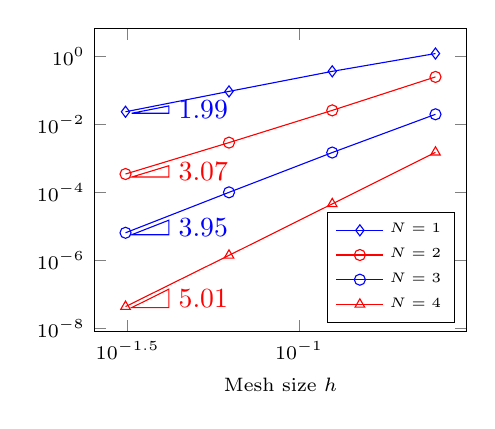
\begin{tikzpicture}
\begin{loglogaxis}[
width=0.52\textwidth,
%height=0.6\textwidth,
%title = {Snell's Law  for an elastic-acoustic interface},
title style = {font=\large},
legend style = {font=\tiny},
xlabel=Mesh size $h$,
%ylabel=$L^2$ Error,
xlabel style= {font=\scriptsize},
ylabel style= {font=\scriptsize},
legend pos = south east,
%ymin=1e-9
]
\addplot[color=blue,mark=diamond] coordinates {
	(0.25,1.21227)	(0.125, 0.36274)	(0.0625,0.0932777)	(0.0312,0.0234593)
};
\addplot[color=red,mark=o] coordinates {
	(0.25,0.248666)	(0.125, 0.0257738)	(0.0625,0.00290105)	(0.0312,0.000345199)
};

\addplot[color=blue,mark=o] coordinates {
	(0.25,0.0197668)	(0.125, 0.00147982)	(0.0625,0.000099811)	(0.0312,0.00000644744)
};
\addplot[color=red,mark=triangle] coordinates {
	(0.25,0.00150798)	(0.125, 0.0000456722)	(0.0625,0.00000139757)	(0.0312,0.0000000433868)
};
\logLogSlopeTriangle{0.2}{0.1}{0.72}{1.99}{blue};
\logLogSlopeTriangle{0.2}{0.1}{0.51}{3.07}{red};
\logLogSlopeTriangle{0.2}{0.1}{0.32}{3.95}{blue};
\logLogSlopeTriangle{0.2}{0.1}{0.08}{5.01}{red};
\legend{$N=1$,$N=2$,$N=3$,$N=4$}
\end{loglogaxis}
\end{tikzpicture}
}
\subfloat[Scholte wave solution]{
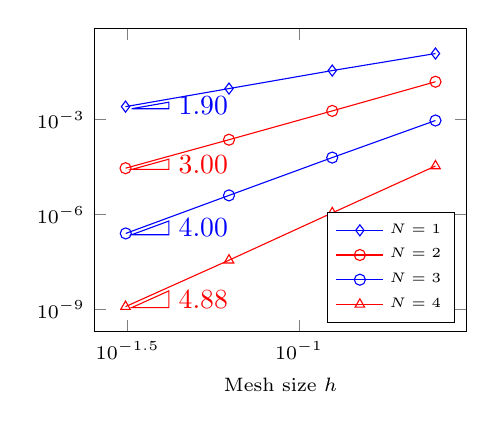
\begin{tikzpicture}
\begin{loglogaxis}[
width=0.52\textwidth,
title style = {font=\large},
legend style = {font=\tiny},
xlabel=Mesh size $h$,
xlabel style= {font=\scriptsize},
ylabel style= {font=\scriptsize},
legend pos = south east,
%ymin=1e-10
]
\addplot[color=blue,mark=diamond] coordinates {
	(0.25,0.124395)	(0.125, 0.0359558)	(0.0625,0.00968633)	(0.0312,0.00259978)
};

\addplot[color=red,mark=o] coordinates {
	(0.25,0.0159341)	(0.125, 0.00190554)	(0.0625,0.000233487)	(0.0312,0.0000292817)
};
\addplot[color=blue,mark=o] coordinates {
	(0.25,0.00094556)	(0.125, 0.0000635446)	(0.0625,0.0000040409)	(0.03125,0.000000253035)
};
\addplot[color=red,mark=triangle] coordinates {
	(0.25,0.0000344301)	(0.125, 0.00000113083 )	(0.0625,0.0000000360469)	(0.0312,0.00000000122477)
};
\logLogSlopeTriangle{0.2}{0.1}{0.735}{1.90}{blue};
\logLogSlopeTriangle{0.2}{0.1}{0.535}{3.00}{red};
\logLogSlopeTriangle{0.2}{0.1}{0.32}{4.00}{blue};
\logLogSlopeTriangle{0.2}{0.1}{0.08}{4.88}{red};
\legend{$N=1$,$N=2$,$N=3$,$N=4$}
\end{loglogaxis}
\end{tikzpicture}}
\vspace{1em}
\caption*{High order convergence of $L^2$ error for acoustic-elastic media.}
}
\end{figure}
}

\frame{
\frametitle{Example with isotropic-anisotropic acoustic-elastic media}
\setcounter{subfigure}{0}
\vspace{-.75em}
\begin{figure}
\centering
\only<1>{
\includegraphics[width=.55\textwidth]{elas_acous3.png}
%\caption*{Problem setup: coupled anisotropic-isotropic elastic-acoustic media.}
}
\only<2>{
\subfloat[$T = 30\mu s$]{\includegraphics[width=.475\textwidth]{T30-homogeneous_nobar.png}}
\hspace{.5em}
\subfloat[$T = 60\mu s$]{\includegraphics[width=.465\textwidth]{T60-homogeneous_nobar.png}}
\caption*{Piecewise constant anisotropic-isotropic acoustic-elastic media.}
}
\only<3>{
\subfloat[$T = 30 \mu s$]{\includegraphics[width=.475\textwidth]{T30-heterogeneous_nobar.png}}
\hspace{.5em}
\subfloat[$T = 60 \mu s$]{\includegraphics[width=.465\textwidth]{T60-heterogeneous_nobar.png}}
\caption*{Piecewise smoothly varying anisotropic-isotropic acoustic-elastic media.}
}
\end{figure}

\let\thefootnote\relax\footnotetext{\tiny Komatitsch, Barnes, Tromp (2000).  \textit{Simulation of anisotropic wave propagation based upon a spectral element method.}}
\let\thefootnote\relax\footnotetext{\tiny Guo, Acosta, Chan (2019).  A weight-adjusted DG method for wave propagation in coupled elastic-acoustic media.}
}


\section{Bernstein-Bezier WADG: high order efficiency }
\frame[noframenumbering]{
  \frametitle{Outline}  
 \tableofcontents[currentsection]
}

\frame{
%\frametitle{Nodal tetrahedra at high order}
\frametitle{Computational costs at high orders of approximation}

%\begin{itemize}
%%\item Hexahedra: tensor product structure $\rightarrow$ $O(N^4)$ vs $O(N^6)$ local cost.
%%\item How do (naively implemented) nodal tetrahedra behave at high order?
%\item 
%\end{itemize}
%\vspace{-.25em}
\begin{center}
Problem: WADG at high orders becomes \textbf{expensive}!
\end{center}
\vspace{-.5em}
\begin{columns}
\begin{column}{.55\textwidth}
\begin{figure}
\centering
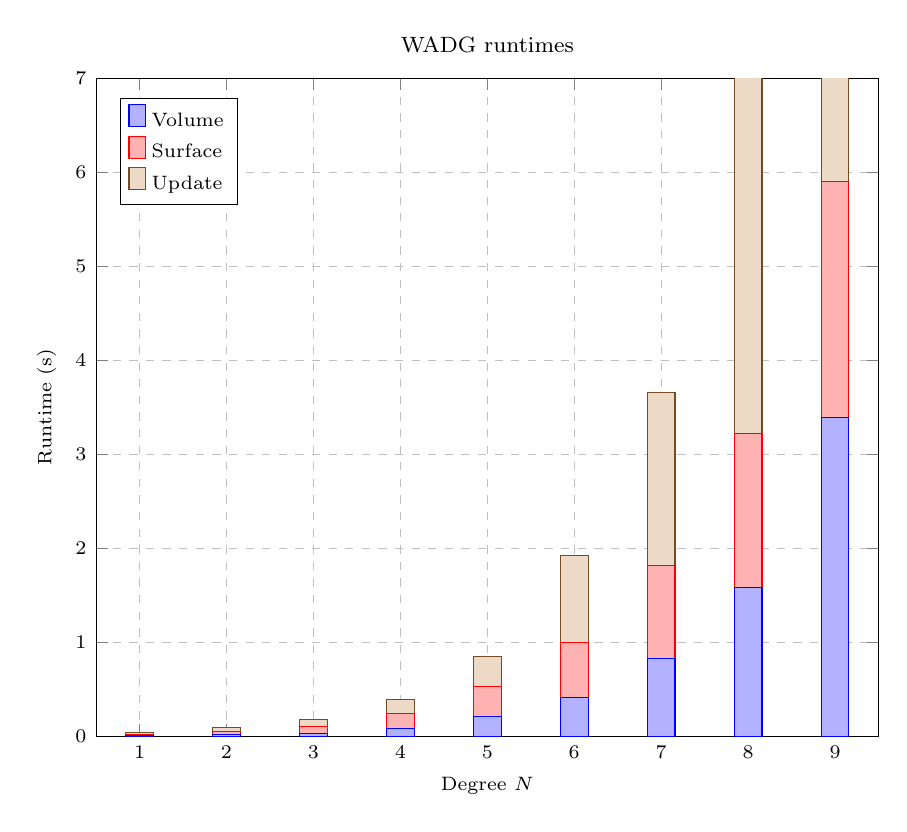
\begin{tikzpicture}
\begin{axis}[
	width=.95\textwidth,
	legend cell align=left,
	%title={Runtime (NPT nodal)},
	title={WADG runtimes},
	xlabel={Degree $N$},
	ylabel={Runtime (s)},
	xmin=.5, xmax=9.5,
	ymin=0,ymax=7,
	ybar stacked,
%	nodes near coords,
	%xmin=.5, xmax=9.5,
	xtick={1,2,3,4,5,6,7,8,9},
	legend pos=north west,
	xmajorgrids=true,
	ymajorgrids=true,
	grid style=dashed,
] 
%nodal runtimes
\addplot coordinates{(1,0.00529)(2,0.0135)(3,0.0302)(4,0.0854)(5,0.206)(6,0.41)(7,0.829)(8,1.58)(9,3.39)};
\addplot coordinates{(1,0.0121)(2,0.0403)(3,0.0722)(4,0.158)(5,0.322)(6,0.587)(7,0.987)(8,1.64)(9,2.51)};
%\addplot coordinates{(1,0.00289997)(2,0.00707789)(3,0.0211354)(4,0.0683213)(5,0.211452)(6,0.530006)(7,1.11929)};
%\addplot coordinates{(1,0.0242951)(2,0.0510198)(3,0.0916193)(4,0.183583)(5,0.397246)(6,1.15212)(7,2.30179)(8,14.2639)};
\addplot coordinates{(1,0.0194361)(2,0.0408158)(3,0.0732955)(4,0.146866)(5,0.317797)(6,0.921698)(7,1.84143)(8,11.4111)(9,21)};


%\addplot coordinates{(1,0.009394)(2,0.025607)(3,0.046205)(4,0.080841)(5,0.142045)(6,0.19389)(7,0.27628)(8,0.381)(9,0.5088)};
%\addplot coordinates{(1,0.026784)(2,0.079407)(3,0.148605)(4,0.324241)(5,0.670045)(6,1.19089)(7,2.09228)(8,3.601)(9,6.4088)};

\legend{Volume, Surface, Update}
%\legend{Volume, Surface}
\end{axis}
\end{tikzpicture}
%\caption*{Per-kernel runtimes for tetrahedra with nodal basis.  Runtimes are recorded for ten RK4 timesteps on a mesh of 98304 elements.}
%\caption*{DG runtimes for 50 timesteps and 98304 elements.}
\caption*{\scriptsize WADG runtimes for 50 timesteps, 98304 elements.}
\end{figure}
\end{column}
\begin{column}{.45\textwidth}
\vspace{-2em}
\begin{itemize}
\item Large \textbf{dense} matrices: $O(N^6)$ work per element.
%\vspace{1em}
%\item High orders usually use tensor-product elements: $O(N^{4})$ vs $O(N^{6})$ cost, but less geometric flexibility.
\vspace{1em}
\item Idea: choose basis such that matrices are \textbf{sparse}.
%\item $O(N^{4})$ vs $O(N^6)$ cost, but less geometric flexibility.
\end{itemize}
\end{column}
\end{columns}
}

\frame{
\frametitle{BBDG: Bernstein-Bezier DG methods}
\setcounter{subfigure}{0}

\begin{itemize}
%\item Hexahedral meshes: $O(N^4)$ with tensor product.
\item<1-> Nodal DG: $O(N^6)$ cost in 3D vs $O(N^3)$ degrees of freedom.
\item<2-> Switch to Bernstein basis: sparse and structured matrices.%, $(d+1)$ non-zeros per row.
\item<4-> Optimal $O(N^3)$ application of differentiation and lifting matrices.
\end{itemize}

\begin{figure}
\begin{overlayarea}{.9\textwidth}{.475\textheight}
\only<1>
{%
\centering
\raisebox{1em}{\subfloat{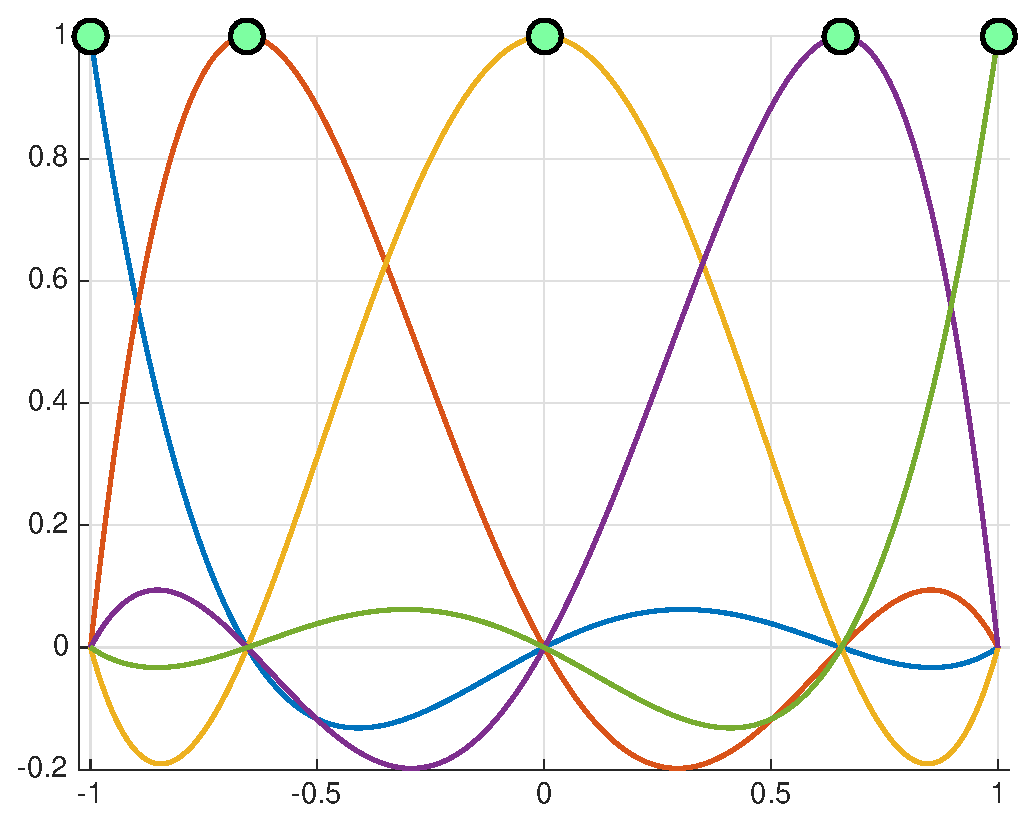
\includegraphics[width=.31\textwidth]{figs/nodal1D.eps}}}
%\hspace{.125em}
\subfloat{\includegraphics[width=.55\textwidth]{figs/nodal2D.png}}
%%\hspace{.125em}
%\subfloat{\includegraphics[width=.375\textwidth]{figs/nodal3D.png}}
\vspace{.1em}
\caption*{Nodal bases in one, two, and three dimensions.}
}%
\only<2>
{%
\centering
\subfloat{\includegraphics[width=.31\textwidth]{figs/bern1D.pdf}}
%\hspace{.125em}
\subfloat{\includegraphics[width=.525\textwidth]{figs/bern2D.png}}
%%\hspace{.125em}
%\subfloat{\includegraphics[width=.375\textwidth]{figs/bern3D.png}}
\vspace{1em}
\caption*{Bernstein bases in one, two, and three dimensions.}
}%
\only<3>
{%
\centering
\subfloat{\includegraphics[height=.425\textheight]{figs/spyD_BB.eps}}
%\hspace{.5em}
%\subfloat{\includegraphics[width=.31\textwidth]{figs/spyD_BB3.eps}}
%\hspace{.5em}
%\subfloat{\includegraphics[width=.31\textwidth]{figs/spyD_BB4.eps}}
\hspace{3em}
\subfloat{\includegraphics[height=.425\textheight]{figs/spyE1.eps}}
%\caption{Sparse Bernstein derivative and degree elevation matrices. }
\caption*{Tetrahedral Bernstein differentiation and degree elevation matrices. }
}%
\only<4>
{%
\centering
\subfloat{\includegraphics[width=.35\textwidth]{figs/bern_lift_1.pdf}}
\subfloat{\includegraphics[width=.35\textwidth]{figs/bern_lift_2.pdf}}
\subfloat{\includegraphics[width=.35\textwidth]{figs/bern_lift_3.pdf}}
\caption*{Optimal $O(N^3)$ complexity ``slice-by-slice'' application of Bernstein lift.}
}%
\end{overlayarea}
\end{figure}
\let\thefootnote\relax\footnotetext{\tiny Chan, Warburton 2017.  {GPU-accelerated Bernstein-Bezier discontinuous Galerkin methods for wave propagation} (SISC).}
}

\frame{
\frametitle{BBDG: efficient volume, surface kernels}

\vspace{-.5em}
%\begin{center}
%Bernstein-Bezier DG achieves $\approx 2\times$ speedup at moderate orders,\\ and up to $\approx 6\times$ speedup at high orders.
%\end{center}
%\begin{center}
%Bernstein-Bezier DG achieves $\approx 2\times$ speedup at moderate orders,\\ and up to $4\times$ speedup at high orders.
%\end{center}
\vspace{-1em}
\begin{figure}
\centering
\only<1>{
\hspace{-1em}
\subfloat{
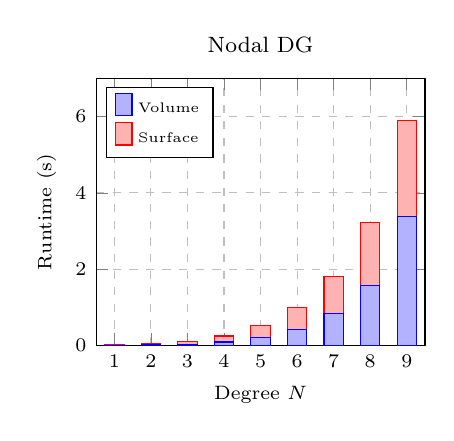
\begin{tikzpicture}
\begin{axis}[
	width=.475\textwidth,
	legend cell align=left,
	title={Nodal DG},
	xlabel={Degree $N$},
	ylabel={Runtime (s)},
	xmin=.5, xmax=9.5,
	ymin=0,ymax=7,
	ybar stacked,
	    bar width=7pt,
	legend style={font=\tiny},	
	xtick={1,2,3,4,5,6,7,8,9},
	legend pos=north west,
	xmajorgrids=true,
	ymajorgrids=true,
	grid style=dashed,
] 
%nodal runtimes
\addplot coordinates{(1,0.00529)(2,0.0135)(3,0.0302)(4,0.0854)(5,0.206)(6,0.41)(7,0.829)(8,1.58)(9,3.39)};
\addplot coordinates{(1,0.0121)(2,0.0403)(3,0.0722)(4,0.158)(5,0.322)(6,0.587)(7,0.987)(8,1.64)(9,2.51)};
%\addplot coordinates{(1,0.009394)(2,0.025607)(3,0.046205)(4,0.080841)(5,0.142045)(6,0.19389)(7,0.27628)(8,0.381)(9,0.5088)};

\legend{Volume, Surface}%, Update}

\end{axis}
\end{tikzpicture}
}
\hspace{1em}
\subfloat{
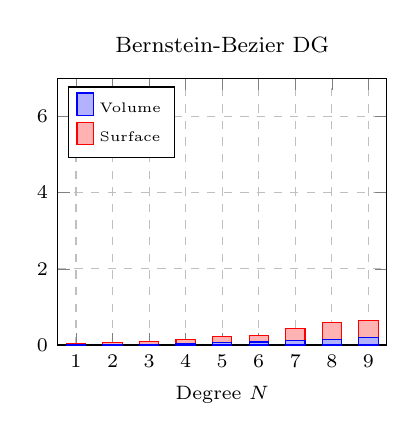
\begin{tikzpicture}
\begin{axis}[
	width=.475\textwidth,
	legend cell align=left,
	title={Bernstein-Bezier DG },
	xlabel={Degree $N$},
	legend style={font=\tiny},	
%	ylabel={Runtime (s)},
	xmin=.5, xmax=9.5,
	ymin=0,ymax=7,
	ybar stacked,
	    bar width=7pt,
	xtick={1,2,3,4,5,6,7,8,9},
	legend pos=north west,
	xmajorgrids=true,
	ymajorgrids=true,
	grid style=dashed,
] 
%bern runtimes
\addplot 
coordinates{(1,0.00564)(2,0.0119)(3,0.0203)(4,0.034)(5,0.0593)(6,0.0791)(7,0.112)(8,0.155)(9,0.204)};
\addplot 
coordinates{(1,3.45E-02)(2,5.15E-02)(3,6.61E-02)(4,1.03E-01)(5,1.76E-01)(6,1.73E-01)(7,3.32E-01)(8,4.48E-01)(9,4.31E-01)};
%\addplot 
%coordinates{(1,0.0093767)(2,0.0255921)(3,0.04623)(4,0.081)(5,0.14229)(6,0.194133)(7,0.277041)(8,0.38163)(9,0.50694)};

\legend{Volume, Surface}%, Update}

\end{axis}
\end{tikzpicture}
}
%\caption*{Per-kernel runtimes for nodal and Bernstein-Bezier bases.  Runtimes are recorded for ten RK4 timesteps on a mesh of 98304 elements.}
%\caption*{Kernel runtimes for Naive nodal, Blocked nodal, and Bernstein-Bezier DG implementations (50 RHS evaluations, 98304 elements).}
%\caption*{Kernel runtimes for Standard nodal, Blocked nodal, and Bernstein-Bezier DG implementations (50 RHS evaluations, 98304 elements).}
%\caption*{DG runtimes for 50 timesteps, 98304 elements.}
}

%% maybe comment out? speedup
%\only<2>{
%\subfloat{
%\begin{tikzpicture}
%\begin{axis}[
%	width=.5\textwidth,
%	legend cell align=left,
%	title={BBDG speedup over nodal DG},
%	xlabel={Degree $N$},
%	ylabel={Speedup},
%	xmin=.5, xmax=9.5,
%	ymin=0,ymax=8,%17.5,	
%        ybar=2*\pgflinewidth,
%    bar width=3pt,
%	xtick={1,2,3,4,5,6,7,8,9},
%	ymin=0,
%	legend pos=north west,
%	legend style={font=\tiny},
%	ymajorgrids=true,
%	grid style=dashed,
%] 
%%speedup V/S
%%\addplot table[x=N, y=V] from \runtimeOptNaive;
%%\addplot table[x=N, y=S] from \runtimeOptNaive;
%\addplot table[x=N, y=V] from \runtimeSpeedupBest;
%\addplot table[x=N, y=S] from \runtimeSpeedupBest;
%%\addplot table[x=N, y=T] from \runtimeOptNaive;
%%\addplot table[x=N, y=Vopt] from \datatable;
%\addplot+[draw=black,line legend, very thick,smooth,dashed] coordinates{(0,1)(10,1)};
%
%%\legend{Volume, Surface, Total, Reference (no speedup)}
%\legend{Volume, Surface}%, Total}%, No speedup}
%\end{axis}
%\end{tikzpicture}
%
%}

%\caption*{Ratio of runtimes of volume/surface kernels and total RHS evaluation using a Bernstein-Bezier basis instead of nodal polynomials.}
%\caption*{Speedups achieved over nodal DG by using a Bernstein-Bezier basis.}
%}

%\caption*{Bernstein-Bezier DG achieves $\approx 2\times$ speedup at moderate orders,\\ and up to $4\times$ speedup at high orders.}
\end{figure}
%\only<1>{\vspace{-.25em}}
%\only<2>{\vspace{-.5em}}
\vspace{-.75em}
\[
\underbrace{\td{\mathbf{u}}{t}}_{\text{Update kernel}} = \underbrace{\mathbf{D}_x \mathbf{u}}_{\text{Volume kernel}} + \underbrace{\sum_{\text{ faces}}\mathbf{L}_f \LRp{\rm flux}}_{\text{Surface kernel}}, \quad \mathbf{L}_f = \mathbf{{M}}^{-1}\mathbf{{M}}_f.
\]
}




%\frame{
%\frametitle{Goal: reduce computational complexity of WADG in 3D}
%
%% note WADG gives explicit expression
%\begin{itemize}
%\item WADG: stable and accurate, but $O(N^6)$ operations per element.
%\vspace{1em}
%\item BBDG: fast $O(N^3)$ evaluation, but requires piecewise constant media
%\vspace{1em}
%\item Exploit continuous WADG approximation: given $u(\bm{x})$, compute 
%\[
%P_N\LRp{ u(\bm{x}) w(\bm{x})}
%\]
%Applying $\bm{M}_w^{-1}$ is always $O(N^6)$ per element, so explicit expression for WADG is a prerequisite for reducing complexity.
%%\vspace{1em}
%%\item Typically discretized using quadrature - can use alternatives.
%\end{itemize}
%}

\frame{
\frametitle{A faster BBWADG update kernel (with Guo)}
\setcounter{subfigure}{0}
\vspace{-1em}
\begin{figure}
\centering
\hspace{-1em}
\subfloat[Exact $c^2$]{\includegraphics[width=.35\textwidth]{figs/cfunEx.png}}
\hspace{-1em}
\subfloat[$M=0$ approximation]{\includegraphics[width=.35\textwidth]{figs/cfun_M0.png}}
\hspace{-1em}
\subfloat[$M=1$ approximation]{\includegraphics[width=.35\textwidth]{figs/cfun_M1.png}}
\end{figure}

\begin{itemize}
%\item $O(N^6)$ update kernel: $\bm{V}_q$ interpolates $u(\bm{x})$ to quadrature points, scale by $c^2(\bm{x})$ at quadrature points, apply $\bm{P}_q$ to project back to $P^N$.
%\item $O(N^6)$ update kernel: multiplication by matrices $\bm{V}_q$ and $\bm{P}_q$.
\item Exploit continuous WADG steps: given $u(\bm{x})$, compute
\[
P_N\LRp{ u(\bm{x}) c^2(\bm{x})}, \qquad P_N = L^2 \text{ projection operator}.
\]
%\vspace{.5em}
\item Our approach: approx.\ $c^2(\bm{x})$ with degree $M$ polynomial, use fast Bernstein algorithms for polynomial multiplication and projection.
\vspace{.5em}
\item Can reuse fast $O(N^3)$ Bernstein-based volume and surface kernels.
\end{itemize}
}

\frame{
\frametitle{BBWADG: effect of approximating $c^2$ on accuracy}

\begin{figure}[h]
\centering
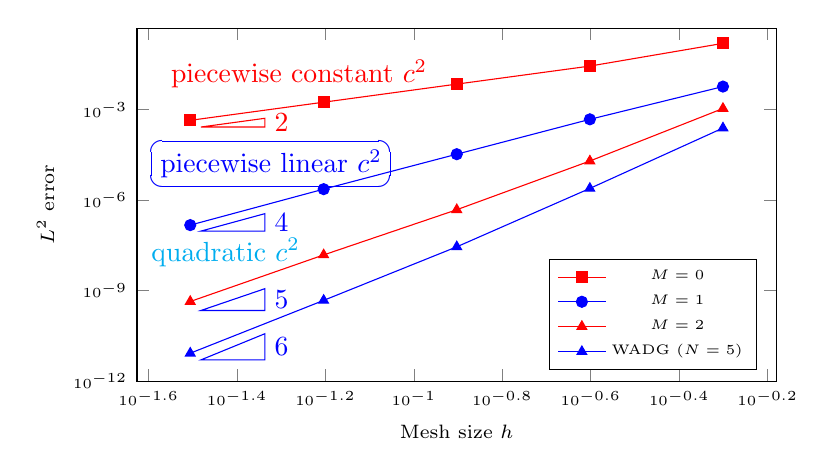
\begin{tikzpicture}
\begin{loglogaxis}[
width=0.8\textwidth,
height=0.5\textwidth,
%title style = {font=\small},
%title = {Convergence of Bernstein-B\'ezier WADG ($N=5$)},
xlabel= Mesh size $h$,
ylabel= $L^2$ error,
ticklabel style = {font=\tiny},
%xtick = data,
%xticklabels={$2$,$3$,$4$,$5$,$6$,$7$,$8$},
ymin=1e-12,ymax=.5,
legend style={font=\tiny},
legend pos = south east
]
\addplot[color=red,mark=square*] coordinates {
(0.5,0.1574265)
(0.25, 0.027776 )
(0.125,0.0070135644)
(0.0625,0.001763477)
(0.0312,0.000441477)
};
\addplot[color=blue,mark=otimes*] coordinates {
(0.5,0.00581413)
(0.25, 0.0004768)
(0.125,0.0000333)
(0.0625, 0.00000230821)
(0.0312,0.000000148265632)
};
\addplot[color=red,mark=triangle*] coordinates {
(0.5,0.0010914511)
(0.25, 0.0000197825)
(0.125,0.00000048003)
(0.0625, 0.000000015234892)
(0.0312,0.000000000434665)
};
\addplot[color=blue,mark=triangle*] coordinates {
(0.5,0.0002451 )
(0.25, 0.0000024406 )
(0.125,0.0000000282596)
(0.0625,0.000000000473564581)
(0.0312,0.000000000008391760)
};
\logLogSlopeTriangle{0.2}{0.1}{0.72}{2}{red};
\logLogSlopeTriangle{0.2}{0.1}{0.425}{4}{blue};
\logLogSlopeTriangle{0.2}{0.1}{0.2}{5}{blue};
\logLogSlopeTriangle{0.2}{0.1}{0.06}{6}{blue};
\node[above,red] at (axis cs: .055,2.5e-3){piecewise constant $c^2$};
\node[above,blue] at (axis cs: .0475,1.25e-6){\ovalbox{piecewise linear $c^2$}};
\node[above,cyan] at (axis cs: .0375,3e-9){quadratic $c^2$};
\legend{$M=0$,$M=1$, $M=2$, WADG ($N=5$)}

\end{loglogaxis}
\end{tikzpicture}
\end{figure}

\begin{center}
Approximating smooth $c^2(\bm{x})$ using $L^2$ projection:\\
\textcolor{red}{$O(h^2)$} for $M=0$, \textcolor{blue}{$O(h^{4})$} for $M = 1$, $O(h^{M+3})$ for $0 < M \leq N-2$. 
\end{center}
}
\frame{
\frametitle{Fast Bernstein polynomial multiplication}
\begin{figure}
\centering
\includegraphics[width=.99\textwidth]{figs/polymult.pdf}
\caption*{Bernstein polynomial multiplication ($M=1$ shown), $O(N^3)$ cost for fixed $M$.}
\end{figure}
}

\frame{
\frametitle{Fast Bernstein polynomial projection}

\begin{itemize}
%\item Polynomial multiplication: $c^2(\bm{x})u(\bm{x}) \in P^{M+N}$.
%\[
%\sum_{j=1}^{M_p} c_j \bm{C}_j \bm{u}.
%\]
\item Given $c^2(\bm{x})u(\bm{x})$ as a degree $(N+M)$ polynomial, apply $L^2$ projection matrix $\bm{P}^{N+M}_N$ to reduce to degree $N$.  
\vspace{.5em}
\item Polynomial $L^2$ projection matrix $\bm{P}^{N+M}_N$ under Bernstein basis: 
\[
\bm{P}^{N+M}_N = %\sum_{j=0}^N c_j\bm{E}_{N-j}^N\LRp{\bm{E}_{N-j}^{N+M}}^T = 
\underbrace{\sum_{j=0}^N c_j\bm{E}_{N-j}^N \LRp{\bm{E}_{N-j}^{N}}^T}_{\tilde{\bm{P}}_N}\LRp{\bm{E}_{N}^{N+M}}^T
\]
\item ``Telescoping'' form of $\tilde{\bm{P}}_N$: \textcolor{red}{$O(N^4)$ complexity}, more GPU-friendly.
\[
\left(c_0\bm{I}+\bm{E}^N_{N-1}\left(c_1\bm{I}+\bm{E}^{N-1}_{N-2}\left(c_2\bm{I}+\cdots\right)\left(\bm{E}^{N-1}_{N-2}\right)^T\right)\left(\bm{E}^N_{N-1}\right)^T\right)
\]
%\item Apply $N$ (sparse) degree elevation matrices $\bm{E}^{j}_{j-1}$: $O(N^4)$ complexity.
\end{itemize}
}

\frame{
\frametitle{Sketch of GPU algorithm for $\tilde{P}_N$}% for $N=3$}
\vspace{-.75em}
\begin{figure}
\centering
\includegraphics[width=.75\textwidth]{figs/bbproj.pdf}
\end{figure}
\vspace{-.5em}
\[
\left(c_0\bm{I}+\bm{E}^N_{N-1}\left(c_1\bm{I}+\bm{E}^{N-1}_{N-2}\left(c_2\bm{I}+\cdots\right)\left(\bm{E}^{N-1}_{N-2}\right)^T\right)\left(\bm{E}^N_{N-1}\right)^T\right)
\]
}



\frame{
\frametitle{BBWADG: computational runtime (3D acoustics)}

\begin{figure}
	\centering
%	\subfloat{
	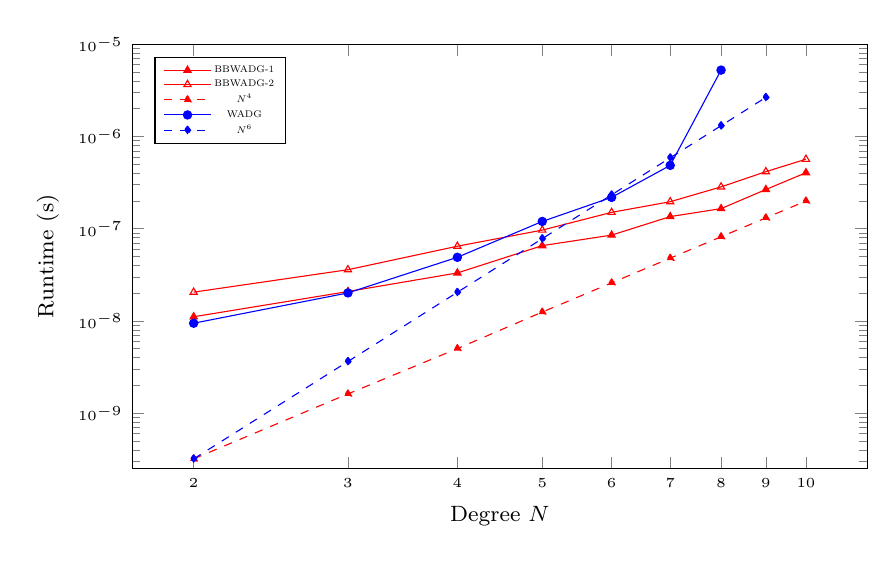
\begin{tikzpicture}
	\begin{loglogaxis}[
	width=0.9\textwidth,
	height=0.575\textwidth,
	%title = { Runtimes per element (update kernel)},
	xlabel=Degree $N$,
	ylabel=Runtime (s),
	xlabel style={font=\footnotesize},
	ylabel style={font=\footnotesize},
	xtick = data,
	ymin=2.5e-10, ymax=1e-5,
	ticklabel style = {font=\tiny},
	xticklabels={$2$,$3$,$4$,$5$,$6$,$7$,$8$,$9$,$10$},
	%legend style={font=\tiny},
	legend pos = north west,
	legend style={nodes={scale=0.5, transform shape}}, 
        %legend image post style={mark=*}
	]
	
	\addplot[color=red,mark=triangle*,mark size=1.5pt] coordinates {
		(2,0.0000000111154)		(3,0.0000000208683)		(4,0.0000000331933)        	        (5,0.0000000656481)		(6,0.000000085396)
		(7,0.000000135523)		(8,0.000000165381)		(9,0.000000266412)	(10,0.000000405157)	};
	\addplot[color=red,mark=triangle,mark size=1.5pt] coordinates {
		(2,0.00000002055)		(3,0.0000000359944)		(4,0.0000000646931)		(5,0.0000000967405)		(6,0.000000150662)
		(7,0.000000196537)		(8,0.000000284467)		(9,0.000000416119)		(10,0.00000056752)	};		
	\addplot[dashed, color=red,mark=triangle*,mark size=1.5pt] coordinates {
		(2,0.00000000032)		(3,0.00000000162)		(4,0.00000000502)		(5,0.00000001250)		(6,0.00000002592)		
		(7,0.00000004802)		(8,0.00000008192)		(9,0.00000013122)		(10,0.00000020000)	};	
	\addplot[color=blue,mark=otimes*,mark size=1.5pt] coordinates {
		(2,0.00000000946015)		(3,0.0000000201553)		(4,0.0000000490578)		(5,0.000000120028)
		(6,0.000000219009)		(7,0.000000487013)		(8,0.00000525304)	};	
	\addplot[dashed, color=blue,mark=diamond*,mark size=1.5pt] coordinates {
		(2,0.00000000032)		(3,0.00000000364)		(4,0.00000002048)		(5,0.00000007812)
		(6,0.00000023328)		(7,0.00000058824)		(8,0.00000131072)		(9,0.00000265720)	};
		
	\legend{BBWADG-1,BBWADG-2,$N^4$, WADG,$N^6$}
	\end{loglogaxis}
	\end{tikzpicture}
\caption*{Per-element runtimes of update kernels for BBWADG vs WADG (acoustic).  We observe an asymptotic complexity of $O(N^4)$ per element for $N\gg 1$.}
\end{figure}
}



\section{Wave propagation in poro-elastic media}
\frame[noframenumbering]{
  \frametitle{Outline}  
 \tableofcontents[currentsection]
}


\frame{
\frametitle{Poro-elastic media (with V.\ de Hoop and Shukla)}
\setcounter{subfigure}{0}
\vspace{-1em}
\begin{figure}
\centering
\subfloat[Orthotropic sandstone]{\includegraphics[width=.35\textwidth]{ortho_sandstone_bz-eps-converted-to.pdf}}
\hspace{2em}
\subfloat[Epoxy glass]{\includegraphics[width=.35\textwidth]{epoxy_glass_bz-eps-converted-to.pdf}}
\end{figure}

\begin{itemize}
\item 3 wave-speed system derived from generalized dynamic Darcy's law by assuming different velocities for solid and fluid particles.
\vspace{.1em}
\item In 3D: 7 stress components (6 stress tensor variables + scalar fluid pressure) and 6 velocity components.  
\end{itemize}

}

\frame{
\frametitle{High order DG vs WADG for poro-elasticity}
\vspace{-2em}
\begin{figure}
\centering
\only<1>{
\setcounter{subfigure}{0}
\subfloat[DG (piecewise constant media)]{\includegraphics[width=.5\textwidth]{DG1.png}}
\subfloat[WADG (high order media)]{\includegraphics[width=.5\textwidth]{WADG1.png}}
\vspace{1em}
\caption*{Degree \rnote{$N = 2$} polynomials, \bnote{$64\times 64$} uniform mesh.  }
}
\only<2>{
\setcounter{subfigure}{0}
\subfloat[DG (piecewise constant media)]{\includegraphics[width=.5\textwidth]{DG2.png}}
\subfloat[WADG (high order media)]{\includegraphics[width=.5\textwidth]{WADG2.png}}
\vspace{1em}
\caption*{Degree \rnote{$N = 4$} polynomials, \bnote{$32\times 32$} uniform mesh.  }
}
\only<3>{
\setcounter{subfigure}{0}
\subfloat[DG (piecewise constant media)]{\includegraphics[width=.5\textwidth]{DG3.png}}
\subfloat[WADG (high order media)]{\includegraphics[width=.5\textwidth]{WADG3.png}}
\vspace{1em}
\caption*{Degree \rnote{$N = 8$} polynomials, \bnote{$16\times 16$} uniform mesh.  }
}
\end{figure}
\begin{center}
WADG is again provably stable and high order accurate.
\end{center}
}

\frame{
\frametitle{Comparison of high order SPECFEM and WADG for a poro-elastic heterogeneous medium}
\vspace{-1.5em}
\setcounter{subfigure}{0}
\begin{figure}
\centering
\subfloat[Vertical solid particle velocity]{
\begin{tikzpicture}
\begin{axis}[enlargelimits=false, axis on top, axis equal image,  width=0.575\textwidth]
\addplot graphics [xmin=0,xmax=4.8,ymin=0,ymax=4.8] {Figure13a-eps-converted-to.pdf};
\node at (axis cs:1.6,2.9)[star,star points=7,draw=black, fill=white, inner sep=0pt,minimum size=7pt]{};
\node at (axis cs:2.0,1.867)[diamond,draw=black, fill=red, inner sep=0pt,minimum size=7pt]{};
\node at (axis cs:3.0,1.8)[draw=black, fill=white, scale=.5] {$\text{(i)}$};
\node at (axis cs:2.5,2.3)[draw=black, fill=white, scale=.5] {$\text{(ii)}$};
\node at (axis cs:1.5,1.9)[draw=black, fill=white, scale=.5] {$\text{(iii)}$};
\node at (axis cs:2.0,2.4)[draw=black, fill=white, scale=.5] {$\text{(iv)}$};
\end{axis}
\end{tikzpicture}
}
\subfloat[Trace showing fast/slow P and S waves]{
\raisebox{1em}{\includegraphics[width=0.575\textwidth]{Figure13b.eps}}
}
%\vspace{1em}
%\caption*{Comparison of SPECFEM and WADG for a heterogeneous poro-elastic medium.}
\end{figure}
}

\frame{
\frametitle{A model poro-elastic reservoir problem}
\begin{figure}
\centering
\only<1>{
\setcounter{subfigure}{0}
\subfloat[Discretized reservoir model ]{\includegraphics[trim={9cm, 1cm, 9cm, 1cm}, clip, height=0.575\textheight]{Figure15a.png}}
\subfloat[Density  model ]{\includegraphics[trim={8cm, 0cm, 7.5cm, 1cm}, clip, height=0.575\textheight]{Figure15b.png}}
}
\only<2>{
\includegraphics[trim={5cm, 1cm, 5cm, 1.25cm}, clip, height=0.75\textheight]{Figure17b.png}
\caption*{Horizontal fluid particle velocity.}
}
\only<3>{
\includegraphics[trim={4cm, 1cm, 7cm, 1cm}, clip, height=0.75\textheight]{Figure16b.png}
\caption*{Horizontal solid particle velocity.}
}
\only<4>{
\setcounter{subfigure}{0}
\subfloat[Vertical solid particle velocity]{\includegraphics[trim={5cm, 1cm, 7cm, 1cm}, clip, height=.48\textheight]{Figure16a.png}}
\hspace{.1em}
\subfloat[Vertical fluid particle velocity]{\includegraphics[trim={4.5cm, 1cm, 7cm, 1cm}, clip, height=.48\textheight]{Figure17a.png}}
}
\end{figure}
}

\frame{
\frametitle{Extensions and current directions}
\vspace{-.75em}
\begin{figure}
\centering
\includegraphics[width=.45\textwidth]{sbp_dcdr.png}
\end{figure}
\vspace{-.75em}
\begin{itemize}
\item Energy stable WADG: immediately extendable to multi-block finite differences through summation-by-parts (SBP) operators.
\vspace{.1em}
\item Stable WADG for moving curved meshes ($r$-adaptivity).
\vspace{.1em}
\item Current: provably stable methods for nonlinear conservation laws.
\end{itemize}

\let\thefootnote\relax\footnotetext{\tiny Kreiss, Scherer (1974). Finite element and finite difference methods for hyperbolic PDEs.}
\let\thefootnote\relax\footnotetext{\tiny Chan, Hewett, Warburton (2017).  {Weight-adjusted DG methods: curvilinear meshes}.}
\let\thefootnote\relax\footnotetext{\tiny Guo, Chan (in preparation).  Weight-adjusted high order DG methods on moving curved meshes.}
}

\frame{
\frametitle{Summary and acknowledgements}

%\vspace{.5em}
\begin{itemize}
\item Weight-adjusted DG: high order accuracy, provable stability, and efficiency in heterogeneous acoustic-elastic and poro-elastic media.  
%\vspace{.25em}
%\item BBWADG: improved efficiency at high orders of approximation.  
\vspace{.5em}
\item This work has been supported by TOTAL E\&P Research and Technology USA and the National Science Foundation under DMS-1712639 and DMS-1719818. 
\end{itemize}
\vspace{.25em}
\begin{center}
Thank you!  Questions?\\
\vspace{.25em}
\includegraphics[width=.125\textwidth]{figs/nsf.jpg}
\end{center}

\let\thefootnote\relax\footnotetext{\tiny Shukla, Chan, deHoop, Jaiswal (2020).  A weight-adjusted DG method for the poroelastic wave equation.}
\let\thefootnote\relax\footnotetext{\tiny Guo, Chan (2020).  {Bernstein-B\'ezier weight-adjusted DG methods for wave propagation in heterogeneous media}.}
\let\thefootnote\relax\footnotetext{\tiny Guo, Acosta, Chan (2019).  A weight-adjusted DG method for wave propagation in coupled elastic-acoustic media.}
\let\thefootnote\relax\footnotetext{\tiny Chan (2018).  Weight-adjusted DG methods: matrix-valued weights and elastic wave prop.\ in heterogeneous media.}
\let\thefootnote\relax\footnotetext{\tiny Chan, Hewett, Warburton (2017).  {Weight-adjusted DG methods: wave propagation in heterogeneous media}.}
\let\thefootnote\relax\footnotetext{\tiny Chan, Warburton (2017).  {GPU-accelerated Bernstein-Bezier discontinuous Galerkin methods for wave propagation}.}
}

%\frame{
%\begin{center}
%The authors thank TOTAL E\&P Research and Technology USA\\
%for their generous support of this work.
%\end{center}
%\let\thefootnote\relax\footnotetext{\tiny Chan, Warburton 2015. {GPU-accelerated Bernstein-Bezier DG methods for wave problems}.}
%\let\thefootnote\relax\footnotetext{\tiny Chan, Warburton 2015.  A short note on a Bernstein-Bezier basis for the pyramid.  (SISC, accepted)}
%\let\thefootnote\relax\footnotetext{\tiny Chan, et al.\ 2016.  {WADG methods I: wave propagation in heterogeneous media}.  In preparation.}
%\let\thefootnote\relax\footnotetext{\tiny Chan, et al.\ 2016.  {WADG methods II: curvilinear meshes}.  In preparation.}
%}
%% =================== extra slides =======================

\begin{frame}[noframenumbering]
\frametitle{Additional slides }

\end{frame}

\frame[noframenumbering]{
\frametitle{Existing approaches: mass lumping}
\vspace{-1em}
\begin{figure}
\centering
\subfloat{\includegraphics[width=.35\textwidth]{figs/SEM_stencil_1.pdf}}
\hspace{2em}
\subfloat{\includegraphics[width=.35\textwidth]{figs/SEM_stencil_2.pdf}}
%\caption{Spectral element stencils for $N = 7$ (orders $N > 10$ not uncommon!).}
\end{figure}

\begin{itemize}
\item DG-SEM: collocate at Gauss-Lobatto (or Gauss) points for a diagonal mass matrix.  $O(N^4)$ total cost in 3D using Kronecker product.
\vspace{.25em}
\item Limited to polynomial quads/hexes! Loss of stability or accuracy when extending to simplices (or prisms, pyramids, or non-polynomials).
\end{itemize}

\let\thefootnote\relax\footnotetext{\tiny Chan, Evans (2018).  {Multi-patch DG-IGA for wave propagation: explicit time-stepping and efficient mass matrix inversion.}}
\let\thefootnote\relax\footnotetext{\tiny Banks, Hagstrom (2016).  On Galerkin difference methods.}
}


\frame[noframenumbering]{
\frametitle{BBWADG: computational runtime (3D elasticity)}

\begin{figure}[]
	\centering
%	\subfloat{
		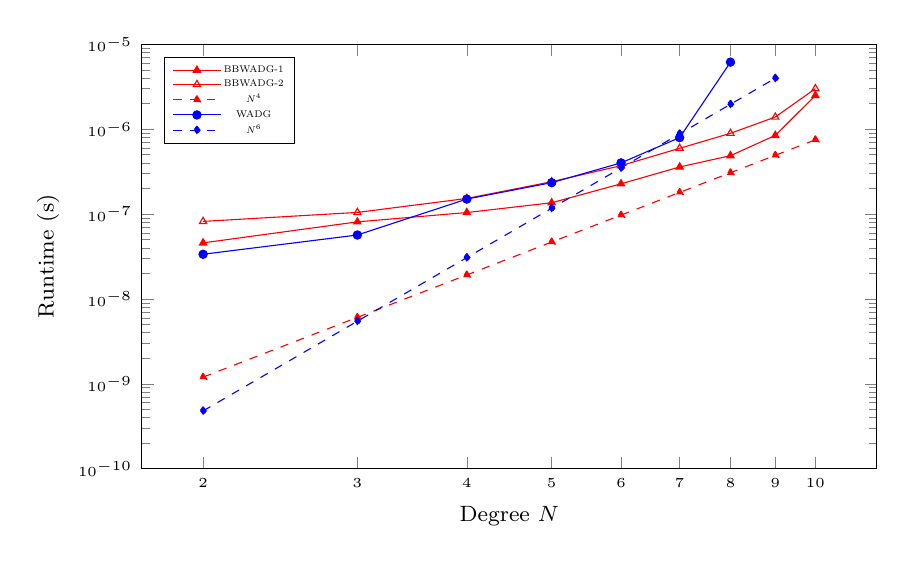
\begin{tikzpicture}
		\begin{loglogaxis}[
		width=0.9\textwidth,
		height=0.575\textwidth,
		%title = { Runtimes per element (update kernel)},
		xlabel=Degree $N$,
		ylabel=Runtime (s),
		xlabel style={font=\footnotesize},
		ylabel style={font=\footnotesize},
		xtick = data,
		ticklabel style = {font=\tiny},
		xticklabels={$2$,$3$,$4$,$5$,$6$,$7$,$8$,$9$,$10$},
		legend pos = north west,
		ymin=1e-10, ymax=1e-5,
	legend style={nodes={scale=0.5, transform shape}}, 
		]
				
		\addplot[color=red,mark=triangle*,mark size=1.5pt] coordinates {
			(2,0.0000000457983)		(3,0.0000000809778)		(4,0.000000104265)		(5,0.00000013602)
		(6,0.000000227247)		(7,0.000000359116)		(8,0.000000487713)		(9,0.00000084492)		(10,0.00000249624)		};
		
		\addplot[color=red,mark=triangle,mark size=1.5pt] coordinates {		
		(2,0.0000000819964)		(3,0.000000104635)		(4,0.000000152827)		(5,0.000000240527)		(6,0.000000371963)
		(7,0.000000595837)		(8,0.000000894296)		(9,0.00000139124)		(10, 0.00000300378)	};		
		\addplot[dashed, color=red,mark=triangle*,mark size=1.5pt] coordinates {
			(2,0.00000000120)			(3,0.00000000607)		(4,0.00000001920)		(5,0.00000004687)	(6,0.00000009720)	
			(7,0.00000018007)			(8,0.00000030720)			(9,0.00000049207)		(10,0.00000075000)		};		
		
		\addplot[color=blue,mark=otimes*,mark size=1.5pt] coordinates {
			(2,0.0000000336389)		(3,0.0000000566972)		(4,0.000000150267)		(5,0.000000234543)		(6,0.000000401095)
		(7,0.000000796524)		(8,0.00000616693)		};
		
		\addplot[dashed, color=blue,mark=diamond*,mark size=1.5pt] coordinates {
			(2,0.00000000048)			(3,0.00000000547)			(4,0.00000003072)			(5,0.00000011719)
			(6,0.00000034992)			(7,0.00000088237)			(8,0.00000196608)			(9,0.00000398580)		};
	
		\legend{BBWADG-1,BBWADG-2, $N^4$, WADG,$N^6$}
		\end{loglogaxis}
		\end{tikzpicture} 
 	\caption*{Per-element runtimes of update kernels for BBWADG vs WADG (elastic).  For $N$ large, heavy use of register memory results in some loss in performance.}
\label{fig:elastime}
\end{figure}
}

\frame[noframenumbering]{
\setcounter{subfigure}{0}
\frametitle{BBWADG: update kernel speedup (3D acoustics)}

\begin{table}
   \centering
   \begin{tabular}{|c||c|c|c|c|c|c|c|} % Column formatting, @{} suppresses leading/trailing space
 \hline
%& $N=2$ 
& $N=3$ & $N=4$ & $N=5$ & $N=6$ & $N=7$  \\
   \hline
WADG  &    1.65e-8  &  3.35e-8 &   6.94e-8 &  1.31e-7 &  3.28e-7  \\
  \hline
BBWADG &   1.81e-8 &  2.59e-8 &   4.22e-8 &   6.16e-8 &  9.79e-8 \\
  \hline
Speedup &    0.9116 &    1.2934 &    1.6445 &    2.1266 &    3.3504 \\
  \hline
\end{tabular}  
\vspace{.5em}
\caption{Achieved speedup for $M=1$} 
\vspace{2em}
	\begin{tabular}{|c||c|c|c|c|c|c|c|} % Column formatting, @{} suppresses leading/trailing space
		\hline
		& $N=3$ & $N=4$ & $N=5$ & $N=6$ & $N=7$ \\
		\hline
		WADG  &          2.02e-8  &  4.91e-8 &   1.20e-7 &  2.19e-7 &  4.87e-7  \\
		\hline
		BBWADG &  3.60e-8  &  6.47e-8 &   9.67e-8 &   1.51e-7 &  1.97e-7 \\
		\hline
		%Speedup & 0.85 &  1.13 & 1.83  & 3.90 & 4.95 & 22.2\\
		Speedup &    0.5611 &    0.7589 &     1.2409 &    1.4503 & 2.4721 \\
		\hline
	\end{tabular}  
	%\vspace{.5em} 
\caption{Achieved speedup for $M=2$}
\label{tab:am2}
\end{table}
}


\bibliographystyle{plain}
{\scriptsize
\bibliography{pyramids}
}

\end{document}
